\documentclass [12pt, a4paper, oneside, titlepage, ngerman]{article}
\usepackage{times}
\usepackage[ngerman]{babel} 
\usepackage[utf8]{inputenc}
\usepackage[T1]{fontenc} 
\usepackage[pdfborder={0 0 0}]{hyperref}
\usepackage{color}
\usepackage{graphicx}
\usepackage{float}
\usepackage{natbib}
\usepackage{enumitem}
\usepackage[printonlyused]{acronym}
\usepackage{url}
\usepackage{geometry} \geometry{a4paper, top=25mm, left=20mm, right=40mm, bottom=20mm} 
\renewcommand{\baselinestretch}{1.5}

\begin {document}



\begin{titlepage}
\Large
\begin{minipage}{\textwidth} \centering \Large
     Duale Hochschule Baden-Württemberg \\  
     Mannheim 
\end{minipage} \vspace{1cm}

\begin{minipage}{\textwidth} \centering \Large
     \textbf{Erste Projektarbeit \\ Erarbeitung eines Lösungsentwurfes für eine IT-Lösung zur Kapazitätsplanung der Kabinencrew}
\end{minipage} \vspace{1cm}

\begin{minipage}{\textwidth} \centering \Large
     \mbox{Studiengang Wirtschaftsinformatik - Sales \& Consulting}\\  \large Bearbeitungszeitraum: 15.05.2017 - 29.08.2017
\end{minipage} \vspace{1cm}


\begin{table}[h!]
\begin{tabular}{ll}
Verfasser: & Julian Garske \\
Matrikelnummer: & 6728241 \vspace{0.5cm} \\ 
Kurs: & WWI SCA16 \\
Studiengangsleiter:& Dr. Frank Koslowski \vspace{0.5cm} \\
Wissenschaftlicher Betreuer: & Günter Stumpf \\ 
Telefon:& 01511 8237778\\ 
Mailadresse:& guenter.stumpf@esosec.de \vspace{0.5cm}\\
Ausbildungsbetrieb: &Lufthansa Systems GmbH \& Co. KG \\ 
& Am Prime Parc 1 \\ 
& D 65479 Raunheim \vspace{0.5cm}\\
Unternehmensbetreuer: &Berger, Iwan \\ 
Telefon(Firma): &+49 (0)69 696 74135 \\
 Mailadresse(Firma):& iwan.berger@lhsystems.com \\
\end{tabular}
\end{table}



\end{titlepage}

\tableofcontents
\newpage


\pagenumbering{gobble}
\section*{Kurzfassung (Abstract)}
\addcontentsline{toc}{section}{Kurzfassung (Abstract)}
\newpage


\pagenumbering{Roman}
\section*{Abkürzungsverzeichnis}
\addcontentsline{toc}{section}{Abkürzungsverzeichnis}

\begin{acronym}[ LSY / Auftragnehmer ]

\acro {BT} {Beschäftigungstage}
\acro {CDB} {Crew Database}
\acro{CAB} {Compas Cabin}
\acro{CMS} {Crew Management System}
\acro{COC} {Compas Cockpit}
\acro {CP} {Captain}
\acro {FO} {First Officer}
\acro{KG} {Kleingruppe}
%\acrodefplural{KG}[KGs]{Kleingruppen} 
\acro{LSY} {Lufthansa Systems}
\acro {NL/C} {NetLine/Crew}
\acro{PU} {Planungseinheit}

\acro {SFO} {Senior First Officer}
%\acro {VAC} {Urlaubsplanungssystem VAC}


\end{acronym}
\newpage


\addcontentsline{toc}{section}{Abbildungsverzeichnis}
\listoffigures
\newpage

\section*{Anlagenverzeichnis}
\addcontentsline{toc}{section}{Anlagenverzeichnis}
\newpage

\pagenumbering{arabic}
\setcounter{page}{1}
\section{Einleitung}
\subsection {Motivation}

%Durchgehen auf sprachliche Fehler, kritisch Abbildungen begutachten
Bereits seitdem es kommerzielle Passagierflüge gibt, ist eine entsprechende Zuteilung der Besatzung für die Flüge notwendig. Diese Zuteilung kann aber gerade bei immer größer werdenden Fluggesellschaften wie der Lufthansa mit ca. 20.000 Besatzungsmitgliedern zu einer Herausforderung werden. Dabei müssen nicht nur Fehlzeiten wie Urlaub oder Krankheit, sondern auch gesetzliche Vorschriften berücksichtigt werden. Außerdem benötigen unterschiedliche Flugzeuge auch unterschiedliche Qualifikationen. Die Kapazitätsplanung ist daher für jede Airline ein wichtiger Bestandteil des Flugbetriebs. \\
Eine Erweiterung der Kapazitätsplanung ist die Schulungsplanung. Schulungen dauern oft mehrere Wochen und müssen daher langfristig vorher geplant werden, sodass Fehlzeiten ausgeglichen werden können und die Qualifikationen nach der Schulung aktualisiert werden. Das Ziel der Kapazitäts- und Schulungsplanung ist es, immer ausreichend aber nicht zu viel überflüssiges Personal für jeden Flug und jede Schulung bereit zu haben. \\

\noindent Seit 1999 gibt es für die Planung der Piloten des Lufthansa Konzerns das von Lufthansa Systems entwickelte System \ac{COC}. Dadurch ist für die etwa 5.000 Piloten eine Planung für bis zu 15 Monate in Zukunft möglich. Bis heute wird die Funktionalität dieses Programms regelmäßig erweitert. Anstatt das Ganze per Hand zu berechnen können dadurch Zeit gespart und Fehler minimiert werden. \\
Seit der ersten Veröffentlichung von \ac{COC} besteht die Idee, so etwas auch für die Kabinenbesatzung zu entwickeln. Diese Idee wurde immer wieder aufgegriffen und angesprochen, aber ein Projekt mit einer konkreten Analyse oder Entwicklung wurde nie begonnen. \\

\noindent Letztes Jahr hatte sich die Firma M2P Consulting bereits mit der bestehenden Kapazitätsplanung auseinander gesetzt und geprüft, wie man diese verbessern könne und ob \ac{COC} dafür in Frage käme. Das Ergebnis war, dass kurzfristig zwar das bestehende Tool optimiert werden könne, um die Qualität zu verbessern, langfristig solle es aber durch eine systemseitige Lösung abgelöst werden \cite [S.8-10]{M2P}. %Formulierung?

\subsection {Problemstellung und -abgrenzung}
Bis heute wird die Einteilung der Kabinenbesatzung mithilfe von verschiedenen Excel-Tabellen geplant. Diese über 200 Tabellen enthalten Daten aus unterschiedlichen Quellen, die für die Kapazitätsplanung erforderlich sind. Aufgrund der großen Datenmenge und den Verflechtungen der Tabellen untereinander sind Computerabstürze oder Fehler nichts Ungewöhnliches, was zu doppelter Arbeit und Frust der Planer führt \cite[vgl.][]{Gespraech2}. \\ 

\noindent Nach dem Vorbild von \ac{COC} soll eine automatisierte Kapazitäts- und Schulungsplanung jetzt auch für die Kabine, also die komplette Crew, ermöglicht werden. Im Vordergrund steht dabei erst einmal die Kapazitätsplanung, die in dieser Arbeit behandelt wird. Im ersten Schritt wird dafür die Bestandsrechnung analysiert und angepasst.\\ %ggf. später ergänzen, je nachdem wie weit wir kommen
Als Ausgangspunkt für das Projekt wird \ac{COC} mit Ähnlichkeiten in vielen Teilen des Programms genutzt. Unterschiede gibt es in der Anzahl der Personen und Daten, bei der Gruppenbildung und -einteilung und bei einigen Prämissen. Die Vorstellung von dem Ergebnis ist, dass der Berechnungsalgorithmus ähnlich wie in \ac{COC} auf den neu eingeteilten Gruppen angewendet werden kann. \\

\noindent Besonderer Fokus liegt auf der Integration in die bestehende Systemlandschaft von \ac{COC} und die Entwicklung einer mandantenfähigen Lösung, um mehrere Airlines der Lufthansa Gruppe zu integrieren. Dabei sollen modernere Architekturansätze verwendet werden, um sich von der bereits veralteten Architektur von \ac{COC} loszulösen. \\
Im Anwenderkonzept wird gefordert , dass die Ergebnisse zur Weiterverarbeitung in Excel exportiert werden können. Darüberhinaus sollten die Berechnungsläufe getrennt von \ac{COC} erfolgen, um sich gegenseitig nicht zu beeinträchtigen \cite[vgl. dazu][]{anwenderkonzept}.

\subsection {Ziel der Arbeit} 
Diese Projektarbeit zielt darauf, einen Lösungsentwurf für die Entwicklung eines explorativen Prototyps zur Kapazitätsplanung des Kabinenpersonals zu entwerfen. Daraus sollen vor allem die Anforderungsspezifikationen erkennbar sein. Darüber hinaus wird evaluiert, wie weit \ac{COC} dazu als Vorlage dienen und ob \ac{NL/C} für die Entwicklung hilfreich sein kann. Für die beschriebenen Probleme und Merkmale soll ein Lösungsansatz gefunden werden.

\subsection {Vorgehen}
Zunächst geht es darum, die Anforderungen zu ermitteln und eine Spezifikation zu erstellen. Dafür muss ermittelt werden, wie die Planung bis jetzt funktioniert und welche Anforderungen das zu entwickelnde Programm erfüllen soll. Die Quellen der Anforderungen sind die Stakeholder, das sind in diesem Fall besonders die Planerinnen, die interviewt werden . Sie wissen wie die Planung funktioniert und werden das auf der Grundlage dieser Arbeit entwickelte Programm später anwenden. Die Inhalte der Spezifikation werden mit \ac{COC} verglichen, um Gemeinsamnkeiten und Unterschiede zu ermitteln und zu entscheiden, wie man mit diesen  Unterschieden umgeht. Im Vorderung steht dabei als erstes die Bestandsrechnung. Bestimmte Bereiche des Programms müssen im Vergleich zu \ac{COC} modernisiert werden, vieles kann aber auch so übernommen werden \cite[vgl.][]{Gespraech1}. Auch \ac{NL/C} wird dafür in Betracht gezogen. \\
Die Änderungen werden anschließend konkret umgesetzt und ein genauer Entwurf wird erstellt, der als Vorlage zur Entwicklung des Prototyps dient. Man soll daraus präzise erfassen können, welche Anforderungen wie erfüllt werden müssen und wie das Programm entwickelt werden soll.

\subsection{Bisherige Vorgehensweise}
Bisher gibt es für die Kapazitätsplanung der Kabine noch kein wirkliches Tool. Zwei angestellte der Lufthansa planen die Kapazitäten mithilfe von Excel-Tabelle, die Daten aus unterschiedlichen Quellen enthalten. Dafür verknüpfen sie ca. 220 Tabellen miteinander \cite[vgl.][]{Gespraech2}. \\
Nach M2P Consulting sei "`die Handlungsfähigkeit der Kapazitätsplanung in Bezug auf die zukünftige Herausforderungen stark eingeschränkt"' \cite[S.5]{M2P} und "`deckt keine der definierten Soll-Funktionalitäten der Kapazitätsplanung ausreichend ab"' \cite[S.6]{M2P}. Bei den Soll-Funktionalitäten handelt es sich nach M2P um langfristige Bereederung und Budgetplanung und um mittelfristige Bereederung \cite[vgl.][S.6]{M2P}.

\subsection{Überblick über Compas Cockpit}
\ac{COC} dient als Ausgangspunkt für das Projekt und nur einige Besonderheiten der Kabine müssen angepasst werden, um \ac{COC} so dafür zu übernehmen \cite[vgl.][]{Gespraech1}. Deshalb sind ein Überblick über \ac{COC} und Kenntnisse der wichtigsten Funktionen davon wichtig. Dieser Überblick stammt aus einem betriebsinternen Dokument \cite[vgl.][]{compasdoku}. \\
\ac{COC} ist das zentrale Tool für die Kapazitätsplanung des Cockpitpersonals. Ziel dieser Planung ist es, die richtige Anzahl an Piloten mit passenden Qualifikationen zu einem bestimmten Zeitpunkt auf eine Flote bereitstellen zu können. Das kann kurzfristig gesteuert oder langfristig prognostiziert werden. Diese Planung ist sehr komplex, da sehr viele Einflussfaktoren dort berücksichtigt werden müssen. \\
Um während der Planung den Überblick zu behalten, teilt \ac{COC} jeden Piloten eindeutig in eine \ac{PU} ein, die durch Flugzeugtyp, Flotte, Homebase %Glossar
, Funktion und Subfunction %Glossar
definiert ist. Dadurch kann für jede \ac{PU} für einen bestimmten Zeitraum tagesgenau z.B. der Bestand und Bedarf ermittelt und verglichen werden. \\
Zusätzlich wurde das Programm mehrmals um z.B. die Schulungsplanung erweitert, sodass es mittlerweile aus vier internen Hauptmodulen und 2 angrenzenden Zusatzmodulen besteht. %Iwan fragen
Der Fokus dieser Arbeit liegt auf dem ersten Modul, der sogenannten Deltarechnung, die den Flugprogrammbestand in Verhältnis zu ihrem Bedarf setzt. Dafür muss in \ac{CAB} zuerst die Bestandsrechnung implementiert werden. 

\newpage

\section{Problemanalyse}
\subsection{Datenerhebung}
Wie schon im ersten Gespräch festgestellt \cite[vgl.][]{Gespraech1}, soll \ac{CAB} im Vergleich zu \ac{COC}, das die Daten von etwa 6.000 Piloten verarbeitet, mit Daten von ca. 20.000 Personen umgehen können. Das wöchentliche Formatieren dieser Daten dauert bereits in \ac{COC} einige Stunden, für \ac{CAB} wäre es also ungefähr das Vierfache. Es besteht dabei jedoch das Risiko, dass die Laufzeit eher exponentiell ansteigt. Hinzu kommt, dass die Datenbank nicht lange von \ac{CAB} ausgelastet werden darf, weil auch andere Schnittstellen darauf zugreifen. Eine zu starke Auslastung kann dabei zu großen Problemen in sehr unterschiedlichen Bereichen und Systemen führen. \\
Bei der Erhebung der Daten in \ac{COC} werden von der \ac{CDB}, der zentralen Datenbank, die passenden Daten herausgesucht und dann in eine neue View geladen, sodass sie alle in der passenden Form und tagesgenau für die nächsten 450 Tage vorliegen. \\

\noindent Aus diesem Problem resultiert, dass zur Datenerhebung aus der \ac{CDB} eine neue Architektur benötigt wird, um die fast 20 Jahre alte von \ac{COC} zu ersetzen. Hinzu kommt, dass historisch bedingt in \ac{COC} viel zu viele nicht benötigte Daten angefordert werden, die früher vielleicht genutzt wurden aber mittlerweile keinen Zweck mehr erfüllen \cite[vgl.][]{Gespraech3}. Eine Veränderung des Architekturansatzes zur Datenerhebung setzt dabei natürlich Verständnis der bisherigen Architektur von \ac{COC} voraus.

\subsection{Integration in das COMPAS-Umfeld}
Sobald \ac{CAB} weit genug entwickelt worden ist, soll es, den Anforderungen nach, in das bereits bestehende \ac{COC} eingegliedert werden. Dabei soll eine Auswahl des Programms möglich sein und \ac{CAB} soll als Modul oder Erweiterung von \ac{COC} genutzt werden können \cite[vgl.][S.6]{anwenderkonzept}. Daher muss das neue Programm in das bisherige System integriert werden und darf sich nicht zu stark davon unterscheiden. Der offizielle Grund davon ist, dass für alle Planer, die \ac{COC} nutzen können, auch möglich sein soll, \ac{CAB} zu nutzen. Eigentlich hat der Kunde aber vor, \ac{CAB} als Erweiterung einzubauen, um dafür kein neues Projekt zu starten und Geld zu sparen. Deshalb ist eine ähnliche Anordnung der Buttons und Felder sowie ähnliches Design wesentlich. \\



\subsection{Erfassen der Anforderungen} 
Bei der Anforderungsermittlung geht es darum, die passenden Anforderungen von den Stakeholdern zu ermitteln. In diesem Projekt werden die Anforderungen größtenteils von den Kabinenplanerinnen gestellt, dem sogenannten Fachbereich. \\
Die Herausforderungen bei der Ermittlung sind unterschiedliche und häufig wechselnde Anforderungen. Die Stakeholder kennen sie oft selber nicht genau, sodass sich die Wünsche widersprechen oder durch neue Ideen und Vorschläge ändern.%vgl. Zube
Ein anderer problematischer Teil ist das Sprachverständnis während der Anforderungsermittlung. Der "'Fachbereich [kennt] in den seltensten Fällen die Fachbegriffe des Entwicklers [.] und umgekehrt [...]. Somit ist eine Art 'Übersetzungsprozess' zwischen der Sprache des Fachbereichs und der des Entwicklers notwendig"' \cite[S.319]{Alpar2016} . 
Für den Auftragnehmer bedeutet das eine ständige Hinterfragung aller Details und Fachbegriffe und die Absprache jeder Kleinigkeit mit den Stakeholdern, sodass sie vollständig ihren Anforderungen entsprechen. \\



\subsection{Mehrfachqualifikationen}
Die Zuteilung jeder Person zu einer \ac{PU} ist in \ac{COC} eindeutig.
Im Gegensatz dazu kann die Kabinenbesatzung mehreren Flotten zugeordnet sein. Jedes Kabinenmitglied wird einer sogenannten \ac{KG} zugeteilt, die durch Rolle, Flotten und Homebase definiert ist. Jede Person kann dabei bis zu drei, aber auch weniger Flugzeugtypen haben, für die sie qualifiziert ist \cite[vgl.][]{Gespraech2}. Diese Mehrfachqualifikationen müssen sinnvoll in das Programm mit aufzaufgenommen und strukturiert werden, sodass der Algorithmus von \ac{COC} darauf angewendet werden kann.

%\subsection{Einteilung in eindeutige Gruppen}
%Die einfachste Möglichkeit, mit den im letzten Kapitel genannten Mehrfachqualifikationen umzugehen, wäre die \acp{KG} in \acp{PU} umzuformen. Dadurch wäre es möglich, auf diesen umgeformten \acp{PU} wie in \ac{COC} zu rechnen und man könnte fast das ganze Modell zu übernehmen. Andernfalls wäre ein komplett neuer Ansatz notwendig und der Aufwand für das Projekt würde sich stark erhöhen. Die Schwierigkeit besteht darin, zu ermitteln, ob und falls wie die Einteilung und Umrechnung zu \acp{PU} funktionieren kann.

\newpage

\section {Grundlagen/Methodischer Ansatz}
\subsection{Vorgehen bei der Anforderungsanalyse}
Die Anforderungsanalyse ist der erste Schritt bei fast jedem IT-Projekt. Das Ziel der Analyse ist, "`möglichst vollständige Kundenanforderungen in guter Qualität zu dokumentieren und dabei Fehler möglichst frühzeitig zu erkennen und zu beheben"' \cite[S.11]{PohlRupp2015}. \\
Quelle zur Ermittlung der Anforderungen sind Dokumente, bereits existierende Systeme und hauptsächlich die sog. Stakeholder. Diese sind "`Person[en] oder Organisation[en], die (direkt oder indirekt) Einfluss auf die Anforderungen ha[ben]"'\cite[S.21]{PohlRupp2015}. Gemeint sind damit also alle Menschen, die in irgendeiner Weise mit der Software zu tun haben oder haben werden, z.B. der Kunde, der Nutzer, die Entwickler etc. Durch Interviews lässt sich herausfinden, was sich der Kunde vorstellt und wie die Software funktionieren und aussehen soll. \\
Da der Auftraggeber oft selbst nicht genau weiß, was er will und braucht, ist es die Herausforderung für den Analysten, jedes Detail zu hinterfragen, um die "`wahren Wünsche"' zu ermitteln, die genau seinen Erwartungen entsprechen. 
Der Auftraggeber hat oft selbst kein konkretes Bild vor Augen und kennt die Anforderungen selber nur ungenau. Es ist die Aufgabe des Auftragnehmers, "`durch geschickte Fragen auch unbewusste Anforderungen aufzudecken"'\cite[S.28]{PohlRupp2015} und mit wechselnden Anforderungen umgehen zu können.
Es muss also eine ständige Kommunikation und Zusammenarbeit sichergestellt werden, was nur durch eine erfolgreiche Einbindung der Stakeholder in den Ermittlungsprozess geschehen kann\cite[vgl. S. 33-34]{PohlRupp2015}.

\subsection{Qualitätssicherung der Anforderungen}
"`Grundsätzlich gilt, dass die Produkte aller Tätigkeiten bei der Softwareentwicklung [...] qualitätsgesichert [...] werden müssen"' \cite[S.55]{Winter1999}. Deshalb "`ist es notwendig, die Qualität der entwickelnden Anforderungen zu überprüfen"'\cite[S.95]{PohlRupp2015}, um das bereits beschriebene Problem der Anforderungsermittlung zu lösen. \\
Diese ständige Qualitätssicherung dient dazu, Fehler möglichst früh in dem Softwarelebenszyklus, also den "`Phasen, die ein Softwareprodukt bei seiner Herstellung und dem späteren Einsatz durchläuft"' \cite[S.173]{gabler} zu erkennen und zu beheben. Der Grund dafür ist, dass die Fehlerbehebung in der Softwareentwicklung mit steigendem Projektfortschritt mehr Aufwand verursacht \cite[vgl. S.2]{Hussmann}. Aufwand kann dabei Geld, Zeit, Kosten oder auch andere zu erbringende Leistung oder Einsatz sein. Das Ziel ist daher, Fehler schon möglichst früh in dem Projektverlauf zu beseitigen. \\

\noindent Dieser Aufwand der Fehlerbehebung ist der Grund für die Qualitätssicherung der Anforderungsermittlung und dadurch ist sie so wichtig für den Erfolg eines Projektes. Diese wichtige Rolle wird in dem folgenden Balkendiagramm dargestellt:
\begin{figure}[H]
	\hspace{-2cm}
	\centering
	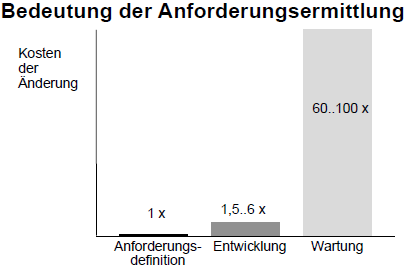
\includegraphics[width=350px,keepaspectratio]{TUDresden.png}
	\caption{Aufwand der Fehlerbehebung}
	\label{img:TUDresden}
\end{figure}
\noindent Das Diagramm beschreibt den Aufwand der Fehlerbehebung in einem Softwareprojekt in Abhängigkeit von dem Projektfortschritt. Der Fortschritt wird dabei als Phasen des Softwarelebenszyklus dargestellt, wobei dieser vereinfacht nur in Anforderungsdefinition, Entwicklung und Wartung aufgeteilt ist. \\

\noindent Wird ein Fehler in der Phase der Anforderungsermittlung oder am Anfang des Projektes behoben, wird der Aufwand dafür mit dem Faktor Eins multipliziert. Sobald ein Fehler gefunden wurde, gilt es die Anforderung zu überarbeiten und ihn einfach zu korrigieren.\\
Während der Entwicklung des Projektes ist der Aufwand meist um das 1,5 bis 6-fache höher. Grund dafür ist, dass Fehler, die sich dann noch in der Software befinden, oft mehrere Bereiche betreffen und viel verändert und berücksichtigt werden muss bevor man sie entgültig beheben kann.\\
Am meisten Aufwand verursacht die Fehlerbehebung, falls der Fehler erst am Ende des Lebenszyklus entdeckt wird. Dabei ist die Software schon in Betrieb und befindet sich in der Wartung. Um dort einen Fehler zu beheben, müssen oft ganze Programmabschnitte verändert werden, damit die Software wieder fehlerfrei läuft. Es hat also große Folgen, wenn ein Teil des Programmes während der Wartung verändert werden muss, weshalb der Aufwand etwa 60 bis 100 mal höher ist als zu Anfang des Projekts. \\
Deshalb ist es so wichtig, die einzelnen Phasen eines Softwarelebenszyklus sorgfältig zu bearbeiten und zu überprüfen, sodass keine Fehler auftreten oder diese schon so früh wie möglich erkannt werden. Es sollte daher nicht zu früh und unvorbereitet mit der Entwicklung begonnen werden.\\
Wie überall gibt es auch hierbei Ausnahmen und Software-Projekte wo dieses Modell nicht zutrifft. Oft lohnt sich der Aufwand in der Analyse jedoch, da "`viele schwerwiegende Fehler in den frühen Phasen IS-Entwicklung [Informationssystem-Entwicklung; Anmerk. d. Verf.] gemacht werdełn"' \cite[S.316]{Alpar2016}. Trotzdem tritt dieser Fehler häufig auf und in vielen Fällen wird zu voreilig mit der Entwicklung angefangen. \\
"`Das Ziel der Überprüfung von Anforderungen ist es [.], Fehler in den dokumentierten Anforderungen zu entdecken"' \cite[S.95]{PohlRupp2015} und sicherzustellen, "`dass die dokumentierten Anforderungen festgelegten Qualitätskriterien genügen, wie z.B. Korrektheit und Abgestimmtheit"' \cite[S.95]{PohlRupp2015}. Diese Qualitätskriterien sind hauptsächlich Inhalt, Dokumentation und Abgestimmtheit. Es wird sich also damit befasst, ob die Anforderungen vollständig, detailliert, passend dokumentiert und mit allen Stakeholdern abgestimmt sind. Für jeden der drei Qualitätsaspekte gibt es damit unterschiedliche Prüfkriterien \cite[vgl.S. 97]{PohlRupp2015}.

\subsubsection{Qualitätsaspekt Inhalt}
"`Der Qualitätsaspekt >>Inhalt<< bezieht sich auf die Überprüfung von Anforderungen auf inhaltliche Fehler"' \cite[S.98]{PohlRupp2015}. Dafür gibt es acht Prüfkriterien\cite[vgl.][S.98]{PohlRupp2015}: 
\begin{description}[font=\itshape]\setlength\itemsep{0em}
\item[Vollständigkeit:] Wurden alle relevanten Anforderungen erfasst?
\item[Korrektheit:] Beschreibt jede Anforderung die dafür notwendigen Informationen?
\item[Verfolgbarkeit:] Können die Anforderungen verfolgt, also z.B. auf die Quelle zurückgeführt werden?
\item[Adäquatheit:] Enthalten die Anforderungen die Bedürfnisse und Wünsche der Stakeholder angemessen?
\item[Konsistenz:] Gibt es Widersprüche zwischen den Anforderungen?
\item[Vorzeitige Entwurfsentscheidungen:] Wurden Entwurfentscheidungen vorweggenommen, die nicht durch Randbedingungen bestimmt sind?
\item[Überprüfbarkeit:] Können Abnahme- und Prüfkriterien anhand der Anforderungen definiert werden?
\item[Notwendigkeit:] Trägt jede Anforderung zu dem definierten Ziel bei?
\end{description}

\subsubsection{Qualitätsaspekt Dokumentation}
Bei der Dokumentation geht es darum, die "`Anforderungen auf Mängel in der Dokumentation bzw. auf Verstöße gegen geltende Dokumentationsvorschriften"'\cite[S.99]{PohlRupp2015} zu überprüfen. Hierbei gibt es folgende vier Prüfkriterien\cite[vlg. S.99f.]{PohlRupp2015}:
\begin{description}[font=\itshape]\setlength\itemsep{0em}
\item[Konformität:] Wurden die Anforderungen in dem vorgeschriebenen Dokumentationsformat strukturiert und in der richtigen Modellierungssprache dokumentiert?
\item[Verständlichkeit:] Können die Anforderungen in dem gegebenen Kontext ggf. mithilfe eines Glossars verstanden werden?
\item[Eindeutigkeit:] Ist eine eindeutige Interpretation möglich?
\item[Konfirmität mit Dokumentationsregeln:] Sind vorgegebene Dokumentationsregeln und -richtlinien eingehalten worden?
\end{description}

\subsubsection{Qualitätsaspekt Abgestimmtheit}
Die Abgestimmtheit stellt sicher, dass keine "'Mängel in der Abstimmung der Anforderungen unter relevanten Stakeholdern"'\cite[S.100]{PohlRupp2015} vorliegen. Auch hierbei gibt es folgende drei Prüfkriterien\cite[vgl. S.100]{PohlRupp2015} :
\begin{description}[font=\itshape]\setlength\itemsep{0em}
\item[Abstimmung:] Wurde jede Anforderung mit relevanten Stakeholdern abgestimmt?
\item[Abstimmung nach Änderungen:] Wurde jede Änderung der Anforderungen auch abgestimmt?
\item[Konflikte:] Wurden alle bekannten Konflikte gelöst?
\end{description}

\subsection{Anforderungskategorisierung}
Anforderungen werden kategorisiert und nach Wichtigkeit eingeteilt. Das ist hilfreich, da die Anforderungen unterschiedlich zur Zufriedenheit der Stakeholder beitragen\cite[vgl. S.24]{PohlRupp2015} . Durch Kategorisierung lassen sie sich leichter einordnen, um Aufwand und Priorität besser abschätzen zu können. \\
In diesem Fall werden die Anforderungen nach dem Kano-Modell kategorisiert. Demnach gibt es drei Kategorien\cite[vgl. S.24]{PohlRupp2015}:
\begin{description} 
\item[Basisfaktoren] sind selbstverständliche unterbewusste Systemmerkmale, die vorausgesetzt werden. 
\item[Leistungsfaktoren] sind bewusste, explizit geforderte Systemmerkmale.
\item[Begeisterungsfaktoren] sind für den Stakeholder unbekannte Systemmerkmale, die er während der Benutzung als angenehme Überraschung entdeckt.
\end{description}
Mit der Zeit werden aus Begeisterungsfaktoren Leistungsfaktoren und aus Leistungsfaktoren Basisfaktoren, da der Nutzer sich an die Merkmale gewöhnt und sie irgendwann voraussetzt. Das Modell lässt sich grafisch darstellen: 

\begin{figure}[H]
	\centering
	\includegraphics{kano.pdf}
	\caption{Grafische Darstellung des Kano-Modells}
	\label{img:kano}
\end{figure}
\noindent Die Grafik zeigt die Zufriedenheit der Stakeholder in Abhängigkeit von dem Erfüllungsgrad der jeweiligen Faktoren. Auf einer dritten Achse wird die Zeit dargestellt, wodurch die Anforderungen die Kategorien wechseln können. \\
Die Basisfaktoren müssen erfüllt sein, um eine massive Unzufriedenheit der Stakeholder zu vermeiden \cite[vgl. S.106]{Kano}. Sie werden vorrausgesetzt und haben daher nur den Nutzen, Unzufriedenheit zu vermeiden Daher verläuft die Funtkion negativ exponentiell. \\
Die Funktion der Leistungsfaktoren verläuft linear und schneidet den Nullpunkt. Diese Faktoren erzeugen proportional Unzufriedenheit, wenn sie nicht erfüllt sind, und Zufriedenheit, wenn sie erfüllt sind \cite[vgl. S.106]{Kano}. \\
Da die Begeisterungsfaktoren vorher den Stakeholdern nicht bekannt sind, kann ihr unzureichender Erfüllungsgrad keine Unzufriedenheit verursachen, da sie nicht erwartet werden oder bekannt sind \cite[vgl. S.106]{Kano}. Das Vorhandensein dieser Faktoren freut jedoch die Stakeholder, wodurch es zu einem überproportionalen Nutzen bei steigender Erfüllung kommt. Deshalb ist die Funktion der Begeisterungsfaktoren linear und erreicht niemals den Wert null oder weniger, aber steigt sehr schnell an. \\

\noindent Es ist ungeklärt, ob man diese Faktoren und ihre Eigenschaften so auf die Anforderungen bei der Erstellung eines Prototyps anwenden kann. Laut Pombergers Definition soll ein explorativer Prototyp ermöglichen, die Vorstellungen der Anwender "`anhand von Anwendungsbeispielen zu prüfen und die gewünschte Funktionalität zu ermitteln"' \cite[S.27]{pomberger2004}, es soll also die Analyse und die Anforderungsspezifikation unterstützen. Das bedeutet, dass der Prototyp nicht alle Anforderungen enthalten kann, besonders die Leistungs- und Begeisterungsfaktoren nicht, und genau im Gegenteil dazu dient, Anforderungen zu ermitteln. \\
Kanos Begeisterungsfaktoren widersprechen zudem dem weit verbreiteten Vorgehen bei einer erfolgreichen Anforderungsanalyse. Wie von Pohl und Rupp beschrieben ist dafür "`eine gute Kommunikation und [...] Qualität der Zusammenarbeit mit den Stakeholdern"' \cite[S.33]{PohlRupp2015} notwendig, um ihn "`erfolgreich in den Ermittlungsprozess einzubinden"' \cite[S.34]{PohlRupp2015}. Durch diese enge Zusammenarbeit werden alle Anforderungen abgesprochen, sodass es keine Begeisterungsfaktoren mehr geben kann.


\subsection{System und Systemkontext abgrenzen}
Die Abgrenzung eines Systemes zu seiner umgebung und zu den Schnittstellen ist essentiell für den Entwurf eines korrekten Produktes. Dafür müssen die System- und Kontextgrenzen bestimmt werden. \\
Dadurch wird Aufwand vermieden, indem bereits vorhandene Funktionen evtl. integriert oder nur in etwas abgeänderter Weise übernommen werden. Außerdem bringt sie Klarheit über die Arten der Informationsgewinnung und -weiterverarbeitung, um Missverständnisse zu vermeiden. Es ist wichtig, "`die Grenzen des Systems zum Systemkontext und die Grenzen des Systemkontexts zur irrelevanten Umgebung zu bestimmen"'\cite[S.20]{PohlRupp2015}, da der Systemkontext "`auch die Anforderungen an das zu entwickelnde System bestimmt"' \cite[S.20]{PohlRupp2015}.

\subsection{Arten und Ziele des Prototypings}
Prototyping beschreibt "`eine Vorgehensweise bei der Softwareentwicklung, bei der nicht sofort ein endgültiges Softwaresystem, sondern zunächst ein oder mehrere Prototypen erstellt werden"' \cite[S.152]{gabler}. Dabei wird nach Kuhrmann zwischen horizontalem und vertikalem Prototyping unterschieden \cite[vgl.][]{Kuhrmann2012}: \\ 
\textbf{Horizontales Prototyping} bezieht sich auf einen bestimmten Bereich der Software, z.B. die Benutzeroberfläche. Der Bezug zu der technischen Funktionalität und der tatsächlichen Implementierung ist dabei nicht gegeben. Nur die eine Ebene des Programms soll vorgestellt werden.\\
Beim \textbf{vertikalen Prototyping} wird ein Ausschnitt komplett in allen Ebenen vollständig implementiert. Diese Art dient zur Demonstration von komplexer Funktionalität.\\

\noindent Darüber hinaus unterscheidet die IEEE %Glossar!
 das Prototyping anhand von Anwendungszwecken \cite[vgl.][S.826]{ieeeprot}: 
\begin{description}
\item[Exploratives Prototyping] wird benutzt, wenn man das Problem und die Anforderungen noch nicht genau kennt. Indem viele Ideen und Ansätze ausprobiert werden, lernt der Entwickler die Arbeit und die Anforderungen des Kunden besser kennen, um die Anforderungen zu identifizieren.
\item[Experimentelles Prototyping] zielt auf das Sammeln von Erfahrungen und Ideen. Der Anwender kann mit dem Prototypen experimentieren, um Ideen an das Programm weiterzuentwickeln und Anforderungen zu konkretisieren. Währenddessen enthält der Entwickler Eindrücke von der Realisierbarkeit des Systems und technischen Herausforderungen.
\item[Evolutionäres Prototyping] stellt die Softwareentwicklung nicht als ein temporäres Projekt, sondern als eine fortlaufende Entwicklung dar. Dabei wird das Programm nach und nach erweitert, wobei der Entwickler eng an der Seite des Anwenders das System immer weiter erweitert.
\end{description}
Die Definition des evolutionären Prototypings widerspricht jedoch der allgemeinen Definition nach \cite{gabler}. Das Ergebnis des explorativen und des experimentellen Prototypings ist ein Prototyp im engeren Sinne, der der Demonstration dient. Dieser wird nach der Erfüllung seiner Aufgaben nicht mehr benötigt \cite[vgl.][S.21]{liggesmeyer2012}. Beim evolutionären Prototyping hingegen entsteht ein Pilotsystem, das der Kern des Produktes ist. Der Prototyp wird also fließend zum laufenden Produkt \cite[vgl.][S.24]{liggesmeyer2012} und ist damit eigentlich kein Prototyp laut Definition mehr.

\newpage

\section {Istanalyse}

\subsection{Bestandsrechnung in Compas Cockpit}
Der aktuelle Algorithmus für die Bestandsrechnung in \ac{COC} ermittelt zuerst den Bruttobestand der Besatzungen \cite[vgl.][S.8]{capfunc}. 
Dazu wird der aktuelle Pilotenbestand mit allen Formen von Zu- und Abgängen z.B. durch Umschulungen, Altersabgänge oder Neueinstellungen und Kündigungen sowie allen bezahlungswirksamen Fehlzeiten wie Teilzeit, Mutterschutz oder Fluguntauglichkeit errechnet \cite[vgl.][S.19]{benutzerhandbuch}. Insgesamt gibt es 16 Kategorien, die hier aber der Übersicht halber nicht alle genannt werden. \\
Von diesem Bruttobestand werden alle weiteren Fehlzeiten, die sich grob in Urlaub und Krankheit einteilen lassen, subtrahiert, was zu dem Nettobestand führt \cite[vgl.][S.8]{capfunc}. \\
Das Ergebnis aller verfügbaren Piloten ergibt sich dann durch die Subtraktion von freien Tagen, die den Piloten zustehen. Auch die Arten und die Berechnung der freien Tage werden hier nicht weiter erläutert. \\
Dadurch ergibt sich der Bestand aller verfügbaren Piloten in \ac{BT}. Diese \ac{BT} lassen sich auf Tages-, Wochen- und Monatsbasis darstellen und zusammenfassen.


\subsection{Anforderungsanalyse- und kategorisierung}
Die Planerinnen formulierten folgende Anforderungen \cite[vgl.]{Gespraech2}:
\begin{description}
\item Basisfaktoren: Es soll ein Programm erstellt werden, dass die Kapazitäts- und später auch die Schulungsplanung automatisch regelt. Dafür müssen vor allem die Gruppen und Untergruppen eingeteilt und dargestellt werden können. Der Zeitraum soll 15 Monate betragen, um die Urlaubsplanung des jeweils kommenden Jahres mit einfließen lassen zu können. Eine Bestandsrechnung wird also benötigt, die später um die Bedarfsrechnung ergänzt werden soll Das Programm wird also nach und nach erweitert bis es in etwa den Funktionalitäten von \ac{COC} entspricht. \\
Der Kunde legt außerdem viel Wert auf Nachvollziehbarkeit. Es soll bei jeder Zelle der Tabellen verstanden werden können, woher die Daten her kommen oder wie sie berechnet werden. Dazu soll es wie bei \ac{COC} die Möglichkeit geben, Reports für einzelne bestimmte Daten abfragen zu können.
\item Leistungsfaktoren: Da es sich um den Entwurf eines Prototyps zur Kapazitätsplanung handelt, ist die Schulungsplanung ein Leistungsfaktor. Dazu gehören auch Bewerbungen für Schulungen. Ein weiterer Leistungsfaktor ist die Bedarfsrechnung. Diese Leistungsfaktoren werden aber später ergänzt, sodass sie nicht Bestandeil dieses Lösungsentwurfs sind. \\
Darüber hinaus wird eine gute Performance erwartet, um die Planung zu erleichtern und Zeit zu sparen.
\item Begeisterungsfaktoren: Modernes Design ist einer der Begeisterungsfaktoren. Dabei ist wünschenswert, das Programm so zu designen, dass sich Cockpit- und Kabinenplaner/innen ersetzen können und die Bedienung und Anordnung der Elemente gleich ist. 
\end{description}
Da sich diese Arbeit aber nur mit der Entwicklung eines Lösungsentwurfs für den Prototypen beschäftigt, stehen die Basisfaktoren im Vordergrund. Die Leistungs- und Begeisterungsfaktoren sind für einen Prototypen erst einmal nur optional. Sie kommen im Verlauf des Projektes dazu. Trotzdem ist eine Analyse davon wichtig, um das System abzugrenzen und Schwerpunkte festzulegen.

\subsection {Die Schnittstelle: Das Crew Management System}
Die Quelle, aus der \ac{COC} die benötigten Daten entnimmt, ist das \ac{CMS} oder genauer gesagt die \ac{CDB}. Unter dem \ac{CMS} wird das gesamte Planungssystem der Lufthansa verstanden, das aus vielen verschiedenen Systemen besteht. Im Mittelpunkt davon steht die \ac{CDB}, wo die Daten zusammen fließen und in der Datenbank gespeichert werden. Es wird also von sehr vielen Seiten aus auf die \ac{CDB} zugegriffen, was ihr sehr viel Leistung und Performance abverlangt. \\
Damit \ac{COC} die passenden Daten in der passenden Form erhalten kann, formatiert (spiegelt) die \ac{CDB} diese Daten wöchentlich, indem sie sie aus allen anderen Tabellen anderer Systeme herausfiltert und dann eine View erstellt, die der benötigten Form entspricht. Das Erstellen dieser View verursacht dabei sehr viel Aufwand und Auslastung der \ac{CDB}.\\
Wenn über \ac{COC} die aktuellen Daten dann angefordert werden, werden sie in eigene Tabellen von \ac{COC} geladen, wo direkt darauf zugegriffen werden kann. Das Aktualisieren der Tabellen aus der View nimmt jedoch nicht viel Zeit in Anspruch, da die Daten nur geladen und nicht verändert oder formatiert werden müssen.



\section{\mbox{Gemeinsamkeiten und Unterschiede zu Compas Cockpit}}
\subsection{Umgang mit Mehrfachqualifikationen}
Nach Absprache des Problems der Mehrfachqualifikationen mit dem Fachbereich haben sich die Anforderungen geändert \cite[vgl.][]{Gespraech4}: \\
Die Anwender haben eine Liste von \acp{PU} erstellt, die wie in \ac{COC} aufgebaut sind, mit dem Unterschied, dass die \acp{PU} mehrere Muster besitzen können. Sie stellen es sich so vor, dass die fest eingeteilten \acp{KG} jeweils manuell einer \ac{PU} vom Nutzer zugeordnet werden können. Diese \acp{PU} sind dann an sich nur Namen, die Bezug zu mehreren \acp{KG} haben, wenn man auf sie zugreift. Diese Zuteilung muss natürlich veränderbar und flexibel sein.

\subsection{Veränderungen bei der Datenspiegelung}
(folgt)
- Problem mit personenbezogenen Daten bei Idee das auf COMPAS Seite zu verlagern\\
- Idee: Verschlüsselung zu CRM-ID -> KG Bildung, Umformen CRM-ID -> Originaldaten nur bei Anfordern\\
- anderer Algorithmus? nur falls es muss

%Daten so auf Compas DB laden, dort View erstellen. Problem: persönliche Daten
%Daten nur bei Anfrage laden, Problem: Ladezeit
%\subsection{Änderungen für die Bestandsrechnung}
%TODO SUBSUBSECTIONS

\newpage

\section {Konkrete Modernisierung und Anpassung von COC}
\newpage

\section {Zusammenfassung und Ausblick}
\newpage

\pagenumbering{gobble}
\addcontentsline{toc}{section}{Literaturverzeichnis}
\bibliographystyle{natdin}

\bibliography{literatur}


\newpage

\pagenumbering{Roman}
\setcounter{page}{4}
\section* {Glossar}
\addcontentsline{toc}{section}{Glossar}
\newpage

\section* {Anlagenverzeichnis}
\addcontentsline{toc}{section}{Anhang}
\newpage

\end{document}

